%- Quintile sorted predicted returns (simonian 2019)
%-OLS
% - summaries for coef attribution
%-RF
% - Summary for feat imp
% compare coefficients between feat imp and ols coef
% Sector rotation strat

\subsection{Hypothesis}
The overarching objective of this study is captured by Research Questions (a) and (b). For Research Question (a), the hypotheses that follow are literature based ex-ante expectations about (i)the incremental contribution of liquidity and sentiment enhancements,(ii) the comparative predictive performance of RF alternatives and (iii) the practicality of applying these specifications to Sector Rotation Strategy.

To address Research Question (a), we first benchmark the traditional Fama-French models. Within the training window we anticipate that all factors in the ($C4F$) and ($FF5$) models will remain statistically significant at the 5\% level. These models should yield low in-sample $R^{2}$, due to its linear nature and non-flexibility to adapt to market changes. This expectation reflects the well-documented risk-pricing roles of market excess return, size, value and momentum premiums, together with profitability and investment effects in the $FF5$ \cite{ff5_2015,cahart_1997}. It is also expected that static OLS specifications will underperform out of sample because their constant beta structure cannot readily accommodate regime shifts in liquidity conditions, investor sentiment or other macroeconomic factors.  When the established linear Fama-French models are enhanced by appending liquidity and sentiment proxies, multicollinearity and over parameterisation are likely to inflate standard errors and obscure economic interpretation. Accordingly, it is predicted that most liquidity and sentiment coefficients will be statistically insignificant, leaving the original $C4F$ and $FF5$ factors
as the only robust drivers. We should also see a reduction both in-sample and out-of-sample fit relative to the linear baselines. The detailed coefficient estimates, significance levels, and economic interpretations for these linear models are intentionally unreported, as doing so would exceed the scope of this study's research questions and would entail presenting an unwieldy number of results across eleven sectors and four model specifications. The full result, however, are available in full in the accompanying GitHub repository.

Random Forest regressions directly target the nonlinearities that handicap OLS, and therefore is the direct comparison for Research Question (a). By aggregating decision trees, RF models can capture higher-order interactions without specifying it in the variables'functional form, while the boostrapping process and random feature subsampling mitigate overfitting provided hyperparameters are tuned via cross-validation. We therefore hypothesise that RF variants of $C4F$ and $FF5$ will deliver higher in-sample $R^{2}$ and lower out-of-sample mean-squared error than their OLS counterparts. Gains should be largest in volatile or growth-oriented sectors where returns are conditional on threshold effects and regime shifts. Notable sectors to look out for include Information Technology, Communication Services, Financials and Real Estate, based on these sectors' descriptive statisitics indicating volatility. Unlike OLS, RF should benefit from the inclusion of a rich set of liquidity and sentiment variables because correlated predictors are essentially decorrelated across trees. Feature-importance measures are expected to highlight the same first-order drivers identified by linear $t$-statistics, but will additionally reveal interaction effects that linear models cannot represent. However, it is important to note that feature importance scores are not directly comparable with $t$ statistics, thus the statistical significance of feature importance scores cannot be directly inferred. 

To statisically compare the forecasting performance between all specifications and variations, we have the following hypotheses for the DM test:
\begin{align}
d_t &= L\bigl(e^{(1)}_t\bigr) \;-\; L\bigl(e^{(2)}_t\bigr), \\[6pt]
H_0: &\quad \mathbb{E}\bigl[d_t\bigr] = 0, \\[4pt]
H_A: &\quad \mathbb{E}\bigl[d_t\bigr] \neq 0.
\end{align}

The null hypothesis indicates that the two forecasting methods have equal expected loss (no difference in predictive accuracy) while the alternative hypothesis states that there is a difference in predictive accuracy.In this specific dataset, it is expected that all RF specifications will outperform their OLS counterparts on a statistically significant level. We expect the same to happen with base vs enhanced of the RF models, albeit at smaller magnitudes. Between the C4F and FF5 variations however, it is not expected to yield a statisically significant difference on all sectors. Of course, in the notable sectors listed above, it is also very likely that in those sectors we could reject the null hypothesis, thereby revealing certain characteristics of these sectors for investors.

For Research Question (b), I hypothesise that ARL applied to the RF based factor forecasts will distill sets of transparent “if-then" rules that will allow for dynamic sector allocations to generate positive active returns relative to the S\&P 500. In particular, we expect that the liquidity and sentiment-enhanced RF-C4F variant will produce the highest cumulative return, alpha, Information Ratio, and Portfolio Sharpe Ratio (at a zero-Sharpe benchmark). This expectation is grounded in recent literature that highlights the pivotal role of momentum, empirical evidence demonstrating that momentum enhances nonparametric forecasting strategies, and studies showing that the FF5 framework is not robust in explaining equity returns \cite{simonian_2019,gu_2020,sarwarff5}. However, it is very likely that for both C4F and FF5, the enhanced variants will outperform their base counterparts in the Sector Rotation strategy.  Enhanced RF-FF5 model will deliver superior risk-adjusted performance to its base counterpart, reflecting the additional information encoded in profitability and investment interactions, while the base RF-C4F model may underperform without these enhancements. Finally, we posit that a constrained implementation—which limits sector deviations from market weights—will preserve the rank order of model performance seen in the unconstrained strategy but offer lower volatility and drawdown, thereby improving the trade-off between active return and active risk.


%For interpretability, comapre the findings of the pseudo beta to the findings of the current literature

\subsection{Model Interpretability}

% - \citeA{simonian_2019} claimed that this could be a good substitute that could help communicate between machine learning models and finance people with a pseudo beta. However, with this data set and with the methods implemented, pseudo beta is unnlikely to be able to translate the findings of Random Forest into actual betas that are able to explain the returns of the assets.

% - It is found that, on all significant instance of any OLS coefficent of variables, RF is always off by 50\% or more. In some cases, we can see a 200 \% difference between the RF and OLS beta.

% - THerefore the notion of attempting to translate between RF betas and OLS is meaningless: This inconsistency goes against the notion of beta for financial experts: have a clear understanding of the drivers of returns and the ability to translate the findings of Random Forest into actual betas that are able to explain the drivers of the assets. Inconsistencies between these models muddy the water, and it does not have a statistical backing of t-tests.

% - However, though for attribution OLS is a better choice, for forecasting tools available are much more diverse and helpful. the magnitude of any variable effect could still be observed through SHAP, PDP and permutation importance so that finance professionals could still have a clear understanding of the drivers of returns.
{Feature Importance}Across the eleven GICS sectors, the RF baseline models display a strikingly uniform importance distribution. In both the C4F and FF5 variants, the excess-market return consistently absorbs the largest share of node split criterion weight (roughly 27-29\%). Size ($SMB$) and value ($HML$) follow at a respectful distance, while momentum ($UMD$) and, in the five-factor specification, profitability ($RMW$) and investment ($CMA$) divide the residual importance fairly evenly. The principal difference between \texttt{C4F} and \texttt{FF5} is minimal: the additional $RMW$ and $CMA$ factors only take a few percentage points from $MKT$, but no variable emerges as a clear new dominant driver. In short, factor contributions are not sector-specific in this analysis, nor does either factor set decisively outshine the other.

Once the models are enhanced with non-traditional predictors, a suprising shift occurs. The sentiment index of \citeA{wurgler_2007} claims close to 10 \% of total importance, displacing $MKT$ as the single most influential determinant of the forest's splits. By contrast, the two liquidity proxies (share turnover and the Amihud illiquidity ratio) exhibit negligible importance, suggesting that their information is either redundant with the traditional factors or consumed by the sentiment measure. Importantly, the inclusion of sentiment alters the importance without changing the uniformity of all the remaining factors. The traditional excess returns still share the bulk of explanatory power, but sentiment supplies an orthogonal source of predictability that the baseline models does not have access to. These findings imply that investor psychology is economically meaningful in sector-level return forecasting, whereas common liquidity metrics, though still share uniform weight in importance, adds less value in non-parametric models.

% For example, if finance practictioners want to look into what drives excess returns the Real Estate sector RF-EN-C4F model, they could look at SHAP values, Partial Dependence Plot (PDP) and Permutation Importance. 
% Automatically generated on 2025-06-29
            \begin{table}[ht]
            \centering
            \caption{\textit{Feature Importances by Sector for RF-BASELINE-C4F-ARL}}
            \label{tab:feature_importance_rf-baseline-c4f-arl}
            \begin{tabular}{lcccc}
            \toprule
            Sector & excess mkt ret & smb & hml & umd \\
            \midrule
            Communication Services & 0.281 & 0.239 & 0.240 & 0.240 \\\\
Consumer Discretionary & 0.281 & 0.237 & 0.243 & 0.238 \\\\
Consumer Staples & 0.287 & 0.238 & 0.237 & 0.238 \\\\
Energy & 0.274 & 0.240 & 0.241 & 0.246 \\\\
Financials & 0.263 & 0.227 & 0.268 & 0.242 \\\\
Health Care & 0.268 & 0.251 & 0.243 & 0.239 \\\\
Industrials & 0.279 & 0.243 & 0.233 & 0.245 \\\\
Information Technology & 0.288 & 0.229 & 0.240 & 0.243 \\\\
Materials & 0.278 & 0.244 & 0.234 & 0.244 \\\\
Real Estate & 0.276 & 0.236 & 0.250 & 0.238 \\\\
Utilities & 0.285 & 0.250 & 0.233 & 0.233 \\\\
            \bottomrule
            \end{tabular}%
            \end{table} 
% Automatically generated on 2025-06-26
            \begin{table}[H]
            \centering
            \caption{\textit{Feature Importances by Sector for RF-BASELINE-FF5-ARL}}
            \label{tab:feature_importance_rf-baseline-ff5-arl}
            \begin{tabular}{p{3.5cm}ccccc}
            \toprule
            Sector & \makebox[1.2cm]{excess mkt ret} & \makebox[0.8cm]{smb} & \makebox[0.8cm]{hml} & \makebox[0.8cm]{rmw} & \makebox[0.8cm]{cma} \\
            \midrule
            Communication Services & 0.235 & 0.198 & 0.199 & 0.189 & 0.179 \\\\
Consumer Discretionary & 0.235 & 0.194 & 0.202 & 0.190 & 0.178 \\\\
Consumer Staples & 0.230 & 0.188 & 0.187 & 0.214 & 0.182 \\\\
Energy & 0.235 & 0.206 & 0.215 & 0.178 & 0.166 \\\\
Financials & 0.236 & 0.189 & 0.252 & 0.164 & 0.158 \\\\
Health Care & 0.218 & 0.204 & 0.192 & 0.206 & 0.179 \\\\
Industrials & 0.237 & 0.200 & 0.204 & 0.191 & 0.168 \\\\
Information Technology & 0.236 & 0.190 & 0.184 & 0.203 & 0.188 \\\\
Materials & 0.234 & 0.206 & 0.202 & 0.190 & 0.168 \\\\
Real Estate & 0.242 & 0.202 & 0.232 & 0.166 & 0.158 \\\\
Utilities & 0.238 & 0.209 & 0.196 & 0.192 & 0.165 \\\\
            \bottomrule
            \end{tabular}%
            \end{table}
% Automatically generated on 2025-06-29
            \begin{table}[H]
            \centering
            \caption{\textit{Feature Importances by Sector for ENHANCED-RF-C4F-ARL (1)}}
            \label{tab:feature_importance_enhanced-rf-c4f-arl_1}
            \begin{tabular}{lcccccccc}
            \toprule
            Sector & \begin{tabular}[c]{@{}c@{}}excess mkt\\ret\end{tabular} & smb & hml & umd & turn & \begin{tabular}[c]{@{}c@{}}turn\\sd\end{tabular} & mvel1 & dolvol \\
            \midrule
            Communication Services & 0.084 & 0.076 & 0.080 & 0.075 & 0.078 & 0.000 & 0.075 & 0.064 \\\\
Consumer Discretionary & 0.084 & 0.075 & 0.077 & 0.078 & 0.079 & 0.000 & 0.084 & 0.063 \\\\
Consumer Staples & 0.094 & 0.074 & 0.072 & 0.074 & 0.074 & 0.000 & 0.075 & 0.071 \\\\
Energy & 0.084 & 0.075 & 0.073 & 0.079 & 0.099 & 0.000 & 0.068 & 0.077 \\\\
Financials & 0.078 & 0.069 & 0.080 & 0.076 & 0.106 & 0.000 & 0.090 & 0.068 \\\\
Health Care & 0.083 & 0.078 & 0.076 & 0.076 & 0.076 & 0.000 & 0.074 & 0.071 \\\\
Industrials & 0.085 & 0.076 & 0.075 & 0.074 & 0.077 & 0.000 & 0.086 & 0.066 \\\\
Information Technology & 0.090 & 0.076 & 0.079 & 0.078 & 0.072 & 0.000 & 0.072 & 0.068 \\\\
Materials & 0.084 & 0.080 & 0.076 & 0.077 & 0.075 & 0.000 & 0.080 & 0.068 \\\\
Real Estate & 0.090 & 0.078 & 0.079 & 0.073 & 0.103 & 0.000 & 0.087 & 0.048 \\\\
Utilities & 0.085 & 0.074 & 0.068 & 0.073 & 0.080 & 0.000 & 0.078 & 0.067 \\\\
            \bottomrule
            \end{tabular}%
            \end{table}
% Automatically generated on 2025-06-29
            \begin{table}[ht]
            \centering
            \caption{\textit{Feature Importances by Sector for ENHANCED-RF-C4F-ARL (2)}}
            \label{tab:feature_importance_enhanced-rf-c4f-arl_2}
            \begin{tabular}{lccccccc}
            \toprule
            Sector & daily illq & zero trade ratio & baspread & enhanced baker & vix close & put call ratio & news sent \\
            \midrule
            Communication Services & 0.070 & 0.000 & 0.068 & 0.052 & 0.132 & 0.068 & 0.077 \\\\
Consumer Discretionary & 0.065 & 0.000 & 0.065 & 0.050 & 0.124 & 0.075 & 0.081 \\\\
Consumer Staples & 0.071 & 0.000 & 0.098 & 0.056 & 0.108 & 0.067 & 0.066 \\\\
Energy & 0.062 & 0.001 & 0.081 & 0.049 & 0.111 & 0.064 & 0.077 \\\\
Financials & 0.057 & 0.005 & 0.085 & 0.040 & 0.105 & 0.064 & 0.076 \\\\
Health Care & 0.079 & 0.003 & 0.082 & 0.054 & 0.107 & 0.070 & 0.068 \\\\
Industrials & 0.066 & 0.001 & 0.072 & 0.049 & 0.124 & 0.067 & 0.081 \\\\
Information Technology & 0.069 & 0.001 & 0.079 & 0.053 & 0.114 & 0.076 & 0.073 \\\\
Materials & 0.068 & 0.000 & 0.078 & 0.052 & 0.114 & 0.068 & 0.081 \\\\
Real Estate & 0.061 & 0.000 & 0.068 & 0.046 & 0.129 & 0.069 & 0.068 \\\\
Utilities & 0.071 & 0.000 & 0.100 & 0.051 & 0.117 & 0.067 & 0.068 \\\\
            \bottomrule
            \end{tabular}%
            \end{table}
% Automatically generated on 2025-06-29
            \begin{table}[ht]
            \centering
            \caption{\textit{Feature Importances by Sector for ENHANCED-RF-FF5-ARL (1)}}
            \label{tab:feature_importance_enhanced-rf-ff5-arl_1}
            \begin{tabular}{lcccccccc}
            \toprule
            Sector & excess mkt ret & smb & hml & rmw & cma & turn & turn sd & mvel1 \\
            \midrule
            Communication Services & 0.081 & 0.074 & 0.073 & 0.068 & 0.066 & 0.070 & 0.000 & 0.069 \\\\
Consumer Discretionary & 0.077 & 0.068 & 0.071 & 0.074 & 0.067 & 0.073 & 0.000 & 0.077 \\\\
Consumer Staples & 0.079 & 0.067 & 0.066 & 0.087 & 0.068 & 0.071 & 0.000 & 0.068 \\\\
Energy & 0.081 & 0.073 & 0.069 & 0.065 & 0.059 & 0.086 & 0.000 & 0.067 \\\\
Financials & 0.077 & 0.064 & 0.079 & 0.059 & 0.059 & 0.102 & 0.000 & 0.080 \\\\
Health Care & 0.074 & 0.071 & 0.071 & 0.082 & 0.067 & 0.071 & 0.000 & 0.069 \\\\
Industrials & 0.080 & 0.070 & 0.066 & 0.070 & 0.063 & 0.071 & 0.000 & 0.080 \\\\
Information Technology & 0.087 & 0.071 & 0.068 & 0.085 & 0.075 & 0.066 & 0.000 & 0.064 \\\\
Materials & 0.076 & 0.079 & 0.069 & 0.074 & 0.064 & 0.067 & 0.000 & 0.073 \\\\
Real Estate & 0.089 & 0.067 & 0.085 & 0.066 & 0.059 & 0.095 & 0.000 & 0.085 \\\\
Utilities & 0.080 & 0.071 & 0.064 & 0.069 & 0.061 & 0.074 & 0.000 & 0.073 \\\\
            \bottomrule
            \end{tabular}%
            \end{table}
% Automatically generated on 2025-06-29
            \begin{table}[H]
            \centering
            \caption{\textit{Feature Importances by Sector for ENHANCED-RF-FF5-ARL (2)}}
            \label{tab:feature_importance_enhanced-rf-ff5-arl_2}
            \begin{tabular}{lcccccccc}
            \toprule
            Sector & dolvol & \begin{tabular}[c]{@{}c@{}}daily\\illq\end{tabular} & \begin{tabular}[c]{@{}c@{}}zero trade\\ratio\end{tabular} & baspread & \begin{tabular}[c]{@{}c@{}}enhanced\\baker\end{tabular} & \begin{tabular}[c]{@{}c@{}}vix\\close\end{tabular} & \begin{tabular}[c]{@{}c@{}}put call\\ratio\end{tabular} & \begin{tabular}[c]{@{}c@{}}news\\sent\end{tabular} \\
            \midrule
            Communication Services & 0.058 & 0.065 & 0.000 & 0.061 & 0.051 & 0.131 & 0.064 & 0.071 \\\\
Consumer Discretionary & 0.057 & 0.060 & 0.000 & 0.059 & 0.047 & 0.124 & 0.071 & 0.076 \\\\
Consumer Staples & 0.063 & 0.064 & 0.000 & 0.088 & 0.050 & 0.107 & 0.062 & 0.059 \\\\
Energy & 0.069 & 0.058 & 0.001 & 0.080 & 0.047 & 0.113 & 0.062 & 0.069 \\\\
Financials & 0.059 & 0.055 & 0.004 & 0.080 & 0.039 & 0.111 & 0.062 & 0.071 \\\\
Health Care & 0.068 & 0.070 & 0.003 & 0.077 & 0.048 & 0.104 & 0.064 & 0.062 \\\\
Industrials & 0.060 & 0.061 & 0.001 & 0.069 & 0.047 & 0.121 & 0.064 & 0.077 \\\\
Information Technology & 0.060 & 0.061 & 0.001 & 0.068 & 0.048 & 0.111 & 0.070 & 0.064 \\\\
Materials & 0.062 & 0.063 & 0.000 & 0.075 & 0.048 & 0.117 & 0.060 & 0.073 \\\\
Real Estate & 0.053 & 0.055 & 0.000 & 0.068 & 0.043 & 0.108 & 0.057 & 0.070 \\\\
Utilities & 0.059 & 0.066 & 0.000 & 0.094 & 0.047 & 0.116 & 0.061 & 0.063 \\\\
            \bottomrule
            \end{tabular}%
            \end{table}

\citeA{simonian_2019} originally proposed the concept of a “pseudo-beta” as a bridge between the predictive strengths of RF and the familiar beta coefficients derived from OLS, arguing that weighting RF variable importances by feature elasticity could yield interpretable analogues of linear factor loadings. From 1998 to 2017, Random Forest models were trained and their RFI were converted into pseudo-beta measures. Although these pseudo-beta coefficients do not carry the same statistical guarantees as OLS regression coefficients, they allow finance practitioners that familiar with OLS betas or PCA loadings to interpret black box ML results in familiar terms. In this framework, a one-unit increase in feature $X$ is associated with a $\beta$-unit change in the target variable $Y$, exactly as in a linear model. Because these pseudo-beta values are denominated in dollars, one must account for the fact that inputs such as excess market returns typically vary by less than 0.1 when interpreting their magnitude.

\begin{landscape}
% Automatically generated on 2025-06-30
        \begin{table}[ht]
        \centering
        \caption{\textit{Pseudo-Beta Statistics by Sector for RF-B-C4F (Part 1)}}
        \label{tab:rfi_statistics_1}
        \begin{tabular}{lcccccc}
        \toprule
        \textbf{Variable} & \textbf{Energy} & \textbf{Materials} & \textbf{Industrials} & \textbf{Consumer Discretionary} & \textbf{Consumer Staples} & \textbf{Health Care} \\
        \midrule
        excess\_mkt\_ret & 0.643 & 0.782 & 0.665 & 0.923 & 0.636 & 0.691 \\
smb & 1.06 & 1.29 & 1.09 & 1.46 & 0.991 & 1.22 \\
hml & 1.38 & 1.61 & 1.36 & 1.95 & 1.28 & 1.53 \\
umd & 0.591 & 0.701 & 0.597 & 0.800 & 0.538 & 0.629 \\
        \bottomrule
        \end{tabular}%
        \end{table}

% Automatically generated on 2025-06-30
        \begin{table}[ht]
        \centering
        \caption{\textit{Pseudo-Beta Statistics by Sector for RF-B-C4F (Part 2)}}
        \label{tab:rfi_statistics_2}
        \begin{tabular}{lccccc}
        \toprule
        \textbf{Variable} & \textbf{Financials} & \textbf{Information Technology} & \textbf{Communication Services} & \textbf{Utilities} & \textbf{Real Estate} \\
        \midrule
        excess\_mkt\_ret & 0.679 & 1.02 & 0.666 & 0.578 & 0.715 \\
smb & 1.10 & 1.53 & 1.06 & 0.952 & 1.14 \\
hml & 1.69 & 2.08 & 1.39 & 1.15 & 1.58 \\
umd & 0.640 & 0.884 & 0.580 & 0.483 & 0.629 \\
        \bottomrule
        \end{tabular}%
        \end{table}
% Automatically generated on 2025-06-30
        \begin{table}[ht]
        \centering
        \caption{\textit{Pseudo-Beta Statistics by Sector for RF-B-FF5 (Part 1)}}
        \label{tab:rfi_statistics_1}
        \begin{tabular}{lcccccc}
        \toprule
        \textbf{Variable} & \textbf{Energy} & \textbf{Materials} & \textbf{Industrials} & \textbf{Consumer Discretionary} & \textbf{Consumer Staples} & \textbf{Health Care} \\
        \midrule
        excess\_mkt\_ret & 0.547 & 0.659 & 0.576 & 0.781 & 0.511 & 0.572 \\
smb & 0.898 & 1.09 & 0.912 & 1.21 & 0.780 & 1.00 \\
hml & 1.22 & 1.39 & 1.21 & 1.64 & 1.01 & 1.23 \\
rmw & 0.538 & 0.695 & 0.600 & 0.817 & 0.615 & 0.701 \\
cma & 0.671 & 0.821 & 0.707 & 1.03 & 0.698 & 0.815 \\
        \bottomrule
        \end{tabular}%
        \end{table}

% Automatically generated on 2025-06-30
        \begin{table}[ht]
        \centering
        \caption{\textit{Pseudo-Beta Statistics by Sector for RF-B-FF5 (Part 2)}}
        \label{tab:rfi_statistics_2}
        \begin{tabular}{lccccc}
        \toprule
        \textbf{Variable} & \textbf{Financials} & \textbf{Information Technology} & \textbf{Communication Services} & \textbf{Utilities} & \textbf{Real Estate} \\
        \midrule
        excess\_mkt\_ret & 0.620 & 0.858 & 0.559 & 0.486 & 0.651 \\
smb & 0.933 & 1.30 & 0.884 & 0.800 & 1.02 \\
hml & 1.61 & 1.63 & 1.16 & 0.975 & 1.52 \\
rmw & 0.560 & 0.958 & 0.584 & 0.510 & 0.581 \\
cma & 0.719 & 1.18 & 0.737 & 0.585 & 0.736 \\
        \bottomrule
        \end{tabular}%
        \end{table}
% Automatically generated on 2025-06-30
        \begin{table}[ht]
        \centering
        \caption{\textit{Pseudo-Beta Statistics by Sector for RF-EN-C4F (Part 1)}}
        \label{tab:rfi_statistics_1}
        \begin{tabular}{lcccccc}
        \toprule
        \textbf{Variable} & \textbf{Energy} & \textbf{Materials} & \textbf{Industrials} & \textbf{Consumer Discretionary} & \textbf{Consumer Staples} & \textbf{Health Care} \\
        \midrule
        excess\_mkt\_ret & 0.189 & 0.229 & 0.198 & 0.280 & 0.200 & 0.218 \\
smb & 0.316 & 0.408 & 0.335 & 0.465 & 0.298 & 0.387 \\
hml & 0.399 & 0.505 & 0.428 & 0.625 & 0.373 & 0.489 \\
umd & 0.181 & 0.214 & 0.178 & 0.265 & 0.161 & 0.204 \\
turn & 6.81e-06 & 4.58e-06 & 6.28e-06 & 5.59e-06 & 7.23e-06 & 7.15e-06 \\
turn\_sd & 0.000 & 0.000 & 0.000 & 0.000 & 0.000 & 0.000 \\
mvel1 & 1.64e-06 & 2.59e-06 & 2.20e-06 & 3.23e-06 & 1.75e-06 & 2.14e-06 \\
dolvol & 0.000 & 0.000 & 0.000 & 0.000 & 0.000 & 0.000 \\
daily\_illq & 1.01 & 0.496 & 1.62 & 1.36 & 1.32 & 2.07 \\
zero\_trade\_ratio & 0.019 & 0.000 & 0.120 & 0.000 & 0.000 & 0.014 \\
baspread & 2.36e-05 & 2.98e-05 & 2.50e-05 & 2.26e-05 & 3.97e-05 & 2.97e-05 \\
enhanced\_baker & -6.35e-05 & -8.19e-05 & -6.68e-05 & -9.66e-05 & -6.94e-05 & -8.27e-05 \\
vix\_close & 2.45e-06 & 3.06e-06 & 2.83e-06 & 4.05e-06 & 2.27e-06 & 2.77e-06 \\
put\_call\_ratio & 2.98e-05 & 1.77e-05 & 2.17e-05 & 3.01e-05 & 2.21e-05 & 3.29e-05 \\
news\_sent & 9.41e-04 & 0.001 & 0.001 & 0.001 & 7.72e-04 & 9.79e-04 \\
        \bottomrule
        \end{tabular}%
        \end{table}

% Automatically generated on 2025-06-30
        \begin{table}[ht]
        \centering
        \caption{\textit{Pseudo-Beta Statistics by Sector for RF-EN-C4F (Part 2)}}
        \label{tab:rfi_statistics_2}
        \begin{tabular}{lccccc}
        \toprule
        \textbf{Variable} & \textbf{Financials} & \textbf{Information Technology} & \textbf{Communication Services} & \textbf{Utilities} & \textbf{Real Estate} \\
        \midrule
        excess\_mkt\_ret & 0.199 & 0.324 & 0.201 & 0.174 & 0.234 \\
smb & 0.329 & 0.516 & 0.342 & 0.283 & 0.378 \\
hml & 0.497 & 0.696 & 0.470 & 0.339 & 0.498 \\
umd & 0.198 & 0.286 & 0.184 & 0.153 & 0.192 \\
turn & 7.64e-06 & 5.09e-06 & 5.51e-06 & 5.79e-06 & 7.47e-06 \\
turn\_sd & 0.000 & 0.000 & 0.000 & 0.000 & 0.000 \\
mvel1 & 2.57e-06 & 2.79e-06 & 1.99e-06 & 1.93e-06 & 2.78e-06 \\
dolvol & 0.000 & 0.000 & 0.000 & 0.000 & 0.000 \\
daily\_illq & 1.10 & 5.41 & 1.73 & 0.293 & 0.175 \\
zero\_trade\_ratio & 0.073 & 0.060 & 0.003 & 0.000 & 0.000 \\
baspread & 3.00e-05 & 3.16e-05 & 1.42e-05 & 4.63e-05 & 2.30e-05 \\
enhanced\_baker & -5.92e-05 & -1.12e-04 & -7.31e-05 & -6.07e-05 & -6.98e-05 \\
vix\_close & 2.64e-06 & 4.02e-06 & 3.11e-06 & 2.34e-06 & 3.27e-06 \\
put\_call\_ratio & 2.14e-05 & 6.12e-05 & 2.26e-05 & 1.41e-05 & 1.03e-05 \\
news\_sent & 0.001 & 0.001 & 0.001 & 7.51e-04 & 9.62e-04 \\
        \bottomrule
        \end{tabular}%
        \end{table}
% Automatically generated on 2025-06-30
        \begin{table}[ht]
        \centering
        \caption{\textit{Pseudo-Beta Statistics by Sector for RF-EN-FF5 (Part 1)}}
        \label{tab:rfi_statistics_1}
        \begin{tabular}{lcccccc}
        \toprule
        \textbf{Variable} & \textbf{Energy} & \textbf{Materials} & \textbf{Industrials} & \textbf{Consumer Discretionary} & \textbf{Consumer Staples} & \textbf{Health Care} \\
        \midrule
        excess\_mkt\_ret & 0.185 & 0.211 & 0.188 & 0.254 & 0.174 & 0.186 \\
smb & 0.314 & 0.411 & 0.308 & 0.420 & 0.275 & 0.335 \\
hml & 0.385 & 0.466 & 0.377 & 0.568 & 0.355 & 0.433 \\
rmw & 0.192 & 0.267 & 0.214 & 0.314 & 0.247 & 0.267 \\
cma & 0.235 & 0.310 & 0.256 & 0.380 & 0.260 & 0.293 \\
turn & 6.02e-06 & 4.14e-06 & 5.82e-06 & 5.13e-06 & 7.15e-06 & 6.35e-06 \\
turn\_sd & 0.000 & 0.000 & 0.000 & 0.000 & 0.000 & 0.000 \\
mvel1 & 1.66e-06 & 2.41e-06 & 2.06e-06 & 2.91e-06 & 1.63e-06 & 1.92e-06 \\
dolvol & 0.000 & 0.000 & 0.000 & 0.000 & 0.000 & 0.000 \\
daily\_illq & 0.974 & 0.466 & 1.53 & 1.25 & 1.22 & 1.77 \\
zero\_trade\_ratio & 0.012 & 0.000 & 0.106 & 0.000 & 0.000 & 0.011 \\
baspread & 2.39e-05 & 2.91e-05 & 2.38e-05 & 2.03e-05 & 3.69e-05 & 2.64e-05 \\
enhanced\_baker & -6.32e-05 & -7.77e-05 & -6.43e-05 & -8.99e-05 & -6.38e-05 & -6.94e-05 \\
vix\_close & 2.55e-06 & 3.17e-06 & 2.79e-06 & 3.99e-06 & 2.30e-06 & 2.57e-06 \\
put\_call\_ratio & 2.99e-05 & 1.59e-05 & 2.11e-05 & 2.84e-05 & 2.09e-05 & 2.86e-05 \\
news\_sent & 8.66e-04 & 0.001 & 9.88e-04 & 0.001 & 7.09e-04 & 8.51e-04 \\
        \bottomrule
        \end{tabular}%
        \end{table}

% Automatically generated on 2025-06-30
        \begin{table}[ht]
        \centering
        \caption{\textit{Pseudo-Beta Statistics by Sector for RF-EN-FF5 (Part 2)}}
        \label{tab:rfi_statistics_2}
        \begin{tabular}{lccccc}
        \toprule
        \textbf{Variable} & \textbf{Financials} & \textbf{Information Technology} & \textbf{Communication Services} & \textbf{Utilities} & \textbf{Real Estate} \\
        \midrule
        excess\_mkt\_ret & 0.197 & 0.310 & 0.191 & 0.166 & 0.248 \\
smb & 0.307 & 0.473 & 0.327 & 0.276 & 0.351 \\
hml & 0.494 & 0.596 & 0.420 & 0.323 & 0.574 \\
rmw & 0.198 & 0.394 & 0.210 & 0.184 & 0.239 \\
cma & 0.262 & 0.465 & 0.270 & 0.217 & 0.284 \\
turn & 7.38e-06 & 4.63e-06 & 4.89e-06 & 5.43e-06 & 7.32e-06 \\
turn\_sd & 0.000 & 0.000 & 0.000 & 0.000 & 0.000 \\
mvel1 & 2.30e-06 & 2.44e-06 & 1.79e-06 & 1.84e-06 & 2.91e-06 \\
dolvol & 0.000 & 0.000 & 0.000 & 0.000 & 0.000 \\
daily\_illq & 1.06 & 4.77 & 1.58 & 0.275 & 0.169 \\
zero\_trade\_ratio & 0.062 & 0.051 & 0.000 & 0.000 & 0.000 \\
baspread & 2.85e-05 & 2.71e-05 & 1.24e-05 & 4.43e-05 & 2.44e-05 \\
enhanced\_baker & -5.83e-05 & -1.00e-04 & -6.93e-05 & -5.67e-05 & -6.86e-05 \\
vix\_close & 2.79e-06 & 3.89e-06 & 3.03e-06 & 2.36e-06 & 2.94e-06 \\
put\_call\_ratio & 2.07e-05 & 5.61e-05 & 2.08e-05 & 1.30e-05 & 8.96e-06 \\
news\_sent & 9.98e-04 & 0.001 & 9.11e-04 & 7.13e-04 & 0.001 \\
        \bottomrule
        \end{tabular}%
        \end{table}
\end{landscape}

% Liquidity risk factors:
% - turn, turn sd, mvel, dolvol, basored, zerotrade, daily illq
% Sentiment factors:
% - news sentiment, enhanced baker, vix
% - The RFI mimic the distribution of factor importance in the feature importance
% - Overall cross sectoral movements are strong for base models factors
% - RF B C4F: Excess market return unit increase for excess return is around 0.5 to 1 Across sectors, we can see that Size and value factor drive the magnitude of excess returns up. Meaning that the dollar in excess returns of smaller cap stocks, investors would also see from 1 to 1.5 (notably the consumer discretionary sector) dollars in excess returns. We see an even higher multiplier in the value factor, especially in IT, meaning that investors could get up to 2 times their investment on under valued firms in this sector. This is understandable, as higher risk = higher rewards. Momentum also have a moderate impact on excess returns
% -RF B ff5: same same but profitability and investment each have almost the same impact as momentum, in which it takes its shares from size and value factors.

% -Enhanced Random Forests, both c4f and ff5: Turn over,market equity, ,vix_close,put_call_ratio, baspread and dollar volume extremely minute effects. Zero trading days zero for some sectors, probably due to a low amount of zero trading days. We could infer that Materials, consumer discret, consumer staples, utilities and real estate have no zero trading days -> active.Amihud illq surprisingly have pretty strong effects on certain sectors. IT is crazy hig, with an additional unit in Amihud illq can mark up excess return up 5 dollars in IT. Followed by health care. Enhanced baker sentiment, have a negative contribution to excess returns{check Ung if it is consistent with lit or not}. News sentiment has particularly high effect on excess return in materials industrials, consumer discretionary, fianncials, IT and communication services

The RF baseline models confirm that the traditional Fama French factors remain the primary drivers of excess returns across sectors. In both the C4F and FF5 specifications, the RFI profile closely tracks the established ordering of factor contribution in the literature.  Market beta still dominates, but the size ($SMB$) and value ($HML$) factors make the largest incremental contributions. The pseudo-beta coefficients suggest that a one unit increase in either factor translates into roughly $0.5$ to $1.0$ dollars of additional monthly excess return in most sectors, rising to $1.5$ in the Consumer Discretionary segment. Momentum ($MOM$) shows a more modest yet systematic effect. When profitability ($RMW$) and investment ($CMA$) are added in $FF5$, their elasticities nearly match that of $MOM$, effectively redistributing importance away from $SMB$ and $HML$ without changing significantly going from sector to sector.

Augmenting the models with liquidity-risk and sentiment variables creates interesting insights. Among the liquidity proxies, turnover ($TURN$), market equity ($ME$), dollar volume ($DVOL$), bid-ask spread ($BASPREAD$), zero-trading days ($ZERODAYS$) and Amihud illiquidity ($ILLQ$)—all but $ILLQ$ contribute negligibly: their RFI weights are close to zero, and $ZERODAYS$ is often inactive in sectors such as Materials, Consumer Discretionary, Consumer Staples, Utilities and Real Estate where trading is continuous. By contrast, a one-unit increase in $ILLQ$ lifts predicted excess returns by up to $5$ dollars in Information Technology and by smaller yet economically meaningful amounts in Health Care, highlighting the reward for bearing illiquidity risk in these sectors. For sentiment factors, the News Sentiment Index consistently shows a stable positive effects, especially in Materials, Industrials, Consumer Discretionary, Financials, Information Technology and Communication Services. This suggesting that favourable information about these sectors and individual companies materially boosts sector-level excess returns. However, it is important to note that the effect is not every economically significant. News Sentiment Scores never go past the range $[-0.5, 0.5]$ and usually increases in 0.05 increments in less volatile periods. Therefore, it is impossible to see a one unit increase in news sentiment, in which we only see a 0.001 dollar increase in excess returns. Short-term market fear indices ($VIX_{\text{close}}$) also exert only marginal influence. However, unique in our set of factor is the  enhanced Baker-Wurgler index ($STV$) consistently subtracts from expected returns, indicating that heightened optimism can potentially depresses future performance. 



\subsection{Model Performance Comparison}
The results of the DM tests are reported in \cref{tab:dm_test_combined}.  For both the traditional C4F and FF5 baselines, every comparison between the random forest (RF) and ordinary least squares (OLS) models is statistically significant at the 99\% level—except in the Financials sector, where significance is 95\%.  Accordingly, we reject the null hypothesis of equal forecast accuracy between OLS and RF across all sectors.  A negative DM statistic indicates that the model listed first in each column header achieves lower mean squared error (i.e.\ superior forecasting accuracy) than the model listed second. Therefore, as hypothesized, RF outperforms OLS in this context. When comparing RF specifications, augmenting the C4F baseline with liquidity and sentiment factors yields statistically significant improvements (at the 95\% level or better) for Energy, Materials, Industrials, Utilities, and Real Estate, but produces no detectable change for Consumer Discretionary, Consumer Staples, Healthcare, IT, or Communication Services. A likely explanation is that the Carhart momentum factor ($MOM$) already coincide with much of the information contained in investor sentiment measures for these high activity sectors. Indeed, the FI tables in \cref{tab:feature_importance_rf-baseline-c4f-arl} and \cref{tab:feature_importance_enhanced-rf-c4f-arl_1} show that sentiment variables,particularly $\mathrm{VIX}_{\text{close}}$,rank among the most important predictors.  Thus, adding explicit sentiment inputs may simply replicate existing momentum patterns, making any forecast improvements insignificant.  This interpretation is consistent with \citeA{schmeling_2009}, who finds that a Baker Wurgler sentiment index adds little predictability in markets where momentum effects are pronounced. \citeA{brown_2005} also document that many indirect sentiment proxies move in tandem with momentum returns. \citeA{lee_2000} further observe that, in the Technology and Consumer Staples sectors, sentiment effects are largely embedded within the Carhart momentum factor \citeA{lee_2000}. Similarly, enhancing the FF5 model with the same factors delivers significant accuracy gains in all sectors except Communication Services and Real Estate. However, existing evidence for this phenomena is less established in the current literature. It can be concluded that adding sentiment and liquidity to RF-B-FF5 does not yield significant improvements in accuracy. With RF-B-C4F showing statisitically significant improvements in Communication Services and Real Estate, it is possible that the profitabililty and investment factors ($RMW$ and $CMA$) in FF5 are capturing dynamics that would otherwise be explained by the liquidity and sentiment variables. 

\cref{tab:baseline_ols_c4f,tab:baseline_ols_ff5} (in the Appendix) reports the forecasting performance for the eight model specifications for each of the 11 sectors. The base OLS specifications provide only minimal explanatory power for daily sector level excess returns. In both the C4F and FF5 variants, the baseline models yield an in-sample $R^{2}$ below 1\%, confirming that a purely linear model cannot train on the nonlinear dynamics of almost 2 decades of the growing equity markets. Although the MSE and mean-absolute-error (MAE) values reported in  are numerically small, this is largely due to the low values of daily excess returns (typically the mean is  $<0.001\%$). Notably, for both the C4F and FF5 variants, the Financial sector (40) and especially Real Estate (60) has a high hold out MSEs (0.003 and 0.01 respectively). Augmenting the regressions with liquidity risks and sentiment factors  improves fit only marginally and Financial/Real Estate errors, while reduced, is still large. Overall, the enhanced OLS models remain vulnerable to market shifts and yield volatile out-of-sample errors, and the results show the limitations of linear factor models for forecasting.

By contrast, the RF frameworks deliver an immediate uplift in predictive accuracy. Even without the enhanced factors, the base RF models (\cref{tab:rf_baseline_c4f,tab:rf_baseline_ff5}) more than six fold the $R^{2}$ obtained with OLS and cut hold out (R)MSE by around 100\% on average. The gains are most striking for Real Estate, where RF achieves the second lowest sectoral hold out performace despite that sector's return volatility and liquidity. When liquidity and sentiment are incorporated (\cref{tab:enhanced_rf_c4f,tab:enhanced_rf_ff5}) the fit improves further, yet the incremental error reduction over the baseline RF is modest. This suggests that the tree ensemble already captures much of the nonlinear interaction between the traditional FF factors and the newly added variables. A contradicting pattern emerges across factor sets: the C4F specification excels in highly volatile sectors (notably 40 and 60), whereas FF5 produces a more uniform errors across the remaining segments. Taken together with the interpretability results outlined in the previous section, these results confirm that RF creates a robust and transparent foundation for the thesis's signal-generation and sector-rotation framework. Furthermore, it could be seen that the models' fit and accuracy increase in out-of-sample performance without overfitting on in-sample fit.


\begin{landscape}
\begin{table}[H]
\centering
\caption{Diebold-Mariano Test Results: Comprehensive Comparison Across Experiments}
\label{tab:dm_test_combined}
\begin{tabular}{lccccccc}
\toprule
Sector & \begin{tabular}[c]{@{}c@{}}RF-B-C4F\\vs RF-EN-C4F\end{tabular} & \begin{tabular}[c]{@{}c@{}}RF-B-FF5\\vs RF-EN-FF5\end{tabular} & \begin{tabular}[c]{@{}c@{}}RF-B-C4F\\vs OLS-B-C4F\end{tabular} & \begin{tabular}[c]{@{}c@{}}RF-B-FF5\\vs OLS-B-FF5\end{tabular} & \begin{tabular}[c]{@{}c@{}}RF-EN-C4F\\vs OLS-EN-C4F\end{tabular} & \begin{tabular}[c]{@{}c@{}}RF-EN-FF5\\vs OLS-EN-FF5\end{tabular} \\
\midrule
Energy & -4.162*** & -1.247 & -5.609*** & -6.122*** & -5.819*** & -5.293*** \\
Materials & -7.245*** & -7.974*** & -5.859*** & -5.791*** & -8.091*** & -8.087*** \\
Industrials & -4.024*** & -6.770*** & -4.411*** & -3.859*** & -6.496*** & -7.008*** \\
Consumer Discretionary & -1.117 & -2.359* & -4.432*** & -3.905*** & -3.821*** & -4.689*** \\
Consumer Staples & -0.547 & -7.022*** & -3.843*** & -4.542*** & -3.601*** & -6.994*** \\
Health Care & -0.714 & -4.447*** & -3.900*** & -4.038*** & -4.081*** & -5.808*** \\
Financials & -4.042*** & -3.124** & -2.394* & -2.571* & -4.233*** & -4.132*** \\
Information Technology & -0.593 & -3.237** & -3.365*** & -2.929** & -3.713*** & -4.141*** \\
Communication Services & -1.781 & -4.619*** & -4.953*** & -4.913*** & -5.294*** & -6.429*** \\
Utilities & 4.723*** & -1.836 & -5.077*** & -4.007*** & -3.394*** & -3.744*** \\
Real Estate & -4.839*** & -0.983 & -4.757*** & -4.196*** & -6.800*** & -3.991*** \\
\bottomrule
\end{tabular}
\begin{tablenotes}
\small
\item Significance levels: *** p $\leq$ 0.001, ** p $\leq$ 0.01, * p $\leq$ 0.05
\end{tablenotes}
\end{table}
\end{landscape}

\subsection{Sector Rotation Strategy}
We evaluate the sector rotation strategy over a hold-out sample of 2018. The strategy's performance is benchmarked against the S\&P500 returns index, which is weighted by market capitalization, computed as the product of share price and total shares outstanding. Many empirical studies benchmark their investment or sector rotation strategies against the S\&P500 due to its status as the primary large-cap U.S. equity market proxy, such as \citeA{sawar_2017} where the authors uses S\&P500 as a benchmark for a sector rotation strategy using FF5 alphas. As detailed in \cref{sec:data}, 2018 was characterized by heightened market volatility and adverse macroeconomic shocks; consequently, the cumulative return of the S\&P500 over this period was $-6.24\%$ \footnote{This paper omits the data point on 30-12-2018 since on 30/12/2018, there are no next day signal to be used for forecasting (next trading day is on 2019). Therefore the reported returns is different. If this data point is included, the cumulative return of the S\&P500 over this period was $-6.24\%$ indeed.}. The cummulative return of the equal-weighted portfolio is reported in \cref{tab:equal_weight} and \cref{fig:equal_weight_cum_ret_plot}. While the S\&P500 weighs every security based on their market capitalization, the equal-weighted portfolio assigns equal weight to each security, every trading day. It can be seen that a passive buy and hold equal-weighted portfolio, though operated at a loss in 2018, still beat the S\&P500 index by 4.79\%. This will be a common theme through out this results section. In 2018, due to market conditions, a negative returns does not mean that the strategy is performing poorly. However, if any strategy yields a positive return, it would be considered an outstanding performance by the model underlying that strategy.

\begin{figure}[H]
    \centering
    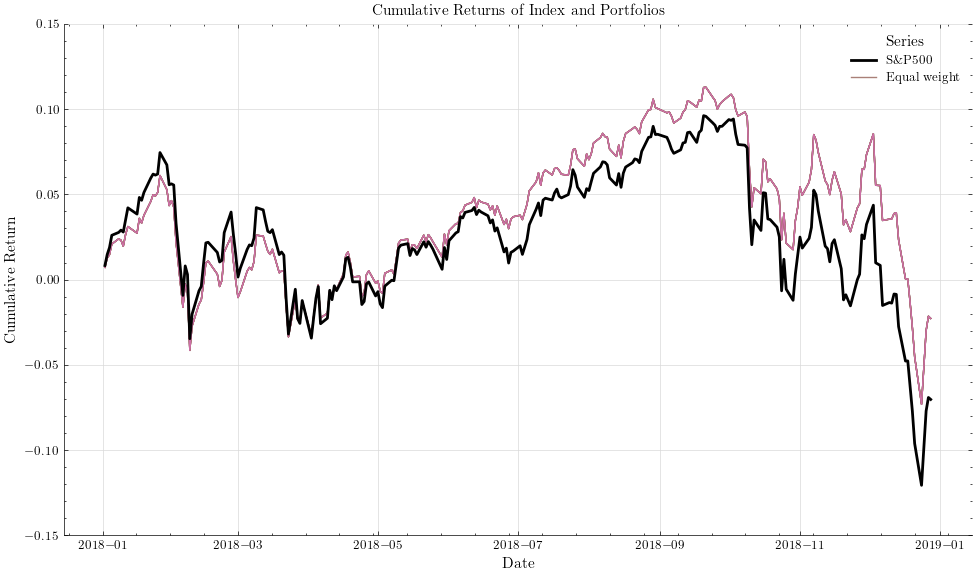
\includegraphics[width=\textwidth]{plots/results/equal_w_cum_ret_plot.png}
    \caption{Cumulative returns of S\&P500 and sector rotation strategies (2018)}\label{fig:eq_w_cum_ret_plot}
\end{figure}


\begin{table}[ht]
\centering
\caption{Descriptive Statistics of Index and Portfolio Returns}
\label{tab:return_stats_1}
\begin{tabular}{lrrrrrrr}
\toprule
{} & \multicolumn{1}{c}{Cumulative} & \multicolumn{1}{c}{Annualised} & \multicolumn{1}{c}{Annualised} & \multicolumn{1}{c}{Alpha} & \multicolumn{1}{c}{Information} & \multicolumn{1}{c}{PSR} & \multicolumn{1}{c}{PSR} \\
{} & \multicolumn{1}{c}{Return} & \multicolumn{1}{c}{Return} & \multicolumn{1}{c}{Volatility} & {} & \multicolumn{1}{c}{Ratio} & \multicolumn{1}{c}{(S*=0)} & \multicolumn{1}{c}{(S*=0.1)} \\
\midrule
S\&P500 & -7.03\% & -7.08\% & 17.06\% & 0.00\% & -- & -- & -- \\
equal\_weight & -2.27\% & -2.29\% & 15.39\% & 4.79\% & 0.29 & 0.92 & 0.45 \\
\bottomrule
\end{tabular}
\end{table}


To gauge risk-adjusted performance of the strategy, we report each portfolio's cumulative return, its active return relative to the S\&P500 (or 'Alpha'), and two spread sensitive statistics: the Information Ratio (IR) and the probabilistic Sharpe Ratio (PSR) at benchmark Sharpe thresholds $S^{*}=0$ and $S^{*}=0.1$. The IR evaluates excess return per unit of tracking-error volatility,

\begin{equation}
\mathrm{IR}=\frac{\mathbb{E}\left[R_{p}-R_{b}\right]}{\sigma\left(R_{p}-R_{b}\right)},
\end{equation}

where $R_{p}$ and $R_{b}$ are portfolio and benchmark returns, respectively, and a higher value signals more efficient investment relative to the risk taken by the investor. For example, an IR of below 0.1 means the strategy generates less than 0.1 units of excess return per unit of tracking error volatility, signaling that its returns are too small relative to their risk to justify strategy implementation. The PSR estimates the posterior probability that the true Sharpe ratio of a strategy exceeds a user-defined benchmark $S^{*}$,

\begin{equation}
\mathrm{PSR}= \Phi\left[\frac{\left(\hat{S}-S^{*}\right)\sqrt{T-1}}{\sqrt{1-\hat{S}^{2}/2}}\right],
\end{equation}
with $\hat{S}$ the sample Sharpe, $T$ the number of observations, and $\Phi(\cdot)$ the standard-normal cdf. Following \citeA{simonian_2019}, we report the PSR at $S^{*}=0$ and $S^{*}=0.1$.


The cumulative return chart for the in \cref{fig:cum_ret_plot} together with the summary statistics in \cref{tab:unconstr} shows the effectiveness of the active unconstrained sector rotation strategies relative to a passive S\&P 500 benchmark buy and hold strategy. While the index declined by 7.03\% over 2018\footnote{Due to ommitted data on 30/12/2018, 2018 period ends on 29/12/2018.}, 7 out of 8 models specifications outperformed the S\&P500 index, and 4 out of 8 specifications made positive returns despite the market conditions. The plot further shows that these active portfolios not only outperformed during the steady upswing through September but also sucessfully adjusted to the sudden sell off and increased volatility from mid-October onward, thereby dampening the loss.

A closer inspection reveals three surprises. First, the top three performers are all RF specifications, yet the fourth-best is an OLS specification. RF-C4f-EN is the best specification, achieving a cumulative return of 5.19\%, translating into an alpha of 12.31\%, an IR of 0.29 and a PSR of 0.97 at the 0.0 Sharpe benchmark.  Second, among RF variants the base FF5 variant outperforms its liquidity and sentiment enhanced variant. Opposite to that, the base RF C4F variant yield negative returns and performed worse than the enhanced OLS FF5 variant, while its enhanced c4f version is the best performing model. Third,  the only portfolio that underperformed the index was the base OLS FF5 (-10.66\%), while its enhanced specification is the only OLS model that generates a postive return, which confirms that both the additional liquidity and sentiment factors are crucial when momentum is missing. Another interesting observation is the RF enhanced models that are C4F variants yield better than their FF5 counterpart. This is probably due to momentum having a particularly strong effect in the macroeconomic environment of 2018, and profitability and investment factors delivered little incremental information.

The constrained strategy,which its statistics are reported in \cref{tab:constr} and \cref{fig:constr_cum_ret_plot}, shows a much more conservative approach to sector weight attribution. Evidently, \cref{fig:constr_cum_ret_plot} shows a much more tight clustering around the S\&P 500, while the unconstrained strategy fans out more. We could see in \cref{tab:constr} that, as expected,the order of the model performance stays exactly the same as the unconstrained model. An advantage of this strategy is that even for OLS models that underperformed against the S\&P500 in unconstrained strategy, the constrained strategy still outperformed the index. Even OLS base FF5 models, which had an active return of -3.58\%, had a positive return of 1.55\% in the constrained strategy. Similarly, OLS base c4f received a bump in active return of 2.2\%, comparing to the unconstrained strategy. What is surprising is that OLS enhanced C4F got lower active returns in the unconstrained strategy (3.2\%), compared to a 4.57\% increase in active returns in the constrained strategy.However, with lower risks comes lower returns. With the top 4 models, the unconstrained strategy got anywhere from 3 to 5\% more active returns than the constrained strategy.

However, implementing these models in actual trading applications requires much more than looking at raw return percentages. Each winning specification shows an IR of only 0.2-0.3, meaning that for every unit of active risk the strategy earns merely 0.2 to 0.3 units of excess return. This level of IR is considered modest at best, since institutional managers typically seek IRs above 0.5 to justify the costs and capacity constraints of active rotation \cite{gratton_2025}. The probabilistic Sharpe ratio at $S^{*} = 0$  with values around 40-60\% implying low confidence that the true Sharpe is larger than zero. In practice, one would prefer PSRs above 90\% at the target Sharpe to ensure robustness against estimation error. It essentially tell investors how likely they will make a positive return relative to the risk taken. In this case, we cannot reject the hypothesis that the true Sharpe ratio is zero. This is understandable given the volatility profile of 2018, where it is extremely uncertain that there would be any positive returns for any strategy. When we refer to the descriptive statistics of 2018, we could see how risky the market is.  Further research, with more computational resources could extend these strategies on a longer horizon (for example, using hold out set of 2016-2018), to have a more accurate outlook on the performance of these underlying models in less volatile periods.



% - Incredible results. Looking at the fig we could see that almost all of  the active strategies are outperforming the buy and hold index strategy. First four models, in a year where Sp500 index loses 7.03%, our strategy were able to hedge against that and even made positive returns. Only one model out of 8 lost against the index
% - In the fig we see that even  the plunge from mid october and volatile times at the end of the year , our models adjusted to that extremely well and generate signals that could hedge against the liquidity risk and sentiment shift
% - Looking closer: top 3 models are rf specification, but extremely surprising that 4rth is ols. Looking deeper in the top 4, c4f enhanced performed best with the cummulative ret =5.19\%, achieving an active return of 12.31\% . surprising that c4f is on top not ff5 {WHY DO YOU THINK c4f is on top not ff5}. even more surprising is that rf_base ff5 seems to beat rf_enhanced_ff5. {WHY IS THIS THE CASE}, with 11.44 active return comapred to 10.65\% active return. Most surpirasing of all, however, is that the 4rth place is not rf but an ols model, specifically ols_en_ff5 {WHY IS THIS POSSIBLE?}

% - Bottom 4 models: rf_base_c4f lost money {WHY enhanced do so good but base lost?}. Contrary to the hypothesis, ols base models performed worse than the ols enhanced, specifically c4f >ff5. Ols_base ff5 is the only one that lost money {WHY?}



\begin{figure}[H]
    \centering
    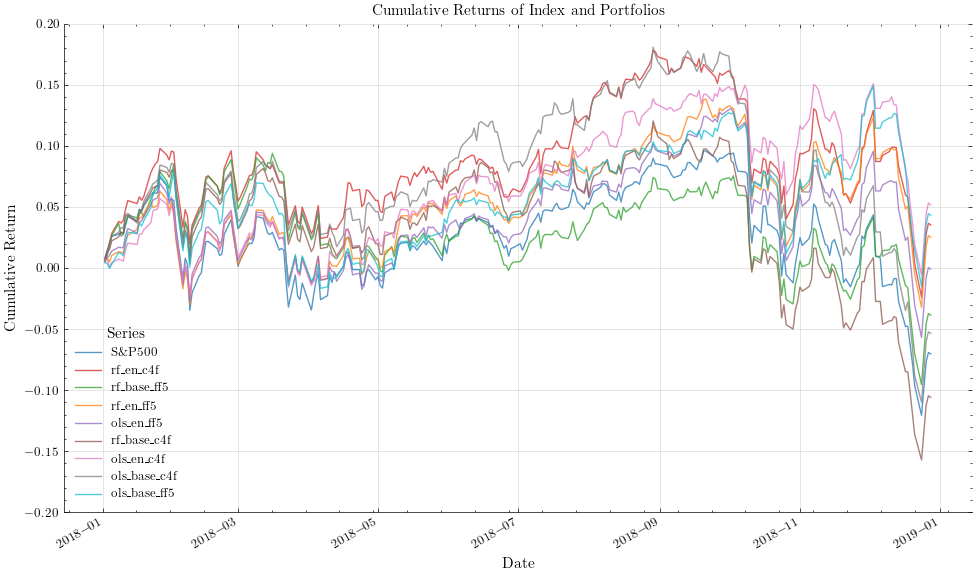
\includegraphics[width=\textwidth]{plots/results/cum_ret_plot.png}
    \caption{Cumulative returns of S\&P500 and sector rotation strategies (2018)}\label{fig:cum_ret_plot}
\end{figure}



% \begin{table}[ht]
% \centering
% \caption{Descriptive Statistics of Index and Portfolio Returns}
% \label{tab:unconstr}
% \begin{tabular}{lrrrrrrr}
% \toprule
% {} & \multicolumn{1}{c}{Cumulative} & \multicolumn{1}{c}{Annualised} & \multicolumn{1}{c}{Annualised} & \multicolumn{1}{c}{Alpha} & \multicolumn{1}{c}{Information} & \multicolumn{1}{c}{PSR} & \multicolumn{1}{c}{PSR} \\
% {} & \multicolumn{1}{c}{Return} & \multicolumn{1}{c}{Return} & \multicolumn{1}{c}{Volatility} & {} & \multicolumn{1}{c}{Ratio} & \multicolumn{1}{c}{(S*=0)} & \multicolumn{1}{c}{(S*=0.1)} \\
% \midrule
% S\&P500 & -7.03\% & -7.08\% & 17.06\% & 0.00\% & -- & -- & -- \\
% rf\_en\_c4f & 5.19\% & 5.23\% & 15.72\% & 12.31\% & 0.29 & 0.97 & 0.61 \\
% rf\_base\_ff5 & 4.33\% & 4.36\% & 16.45\% & 11.44\% & 0.28 & 0.95 & 0.57 \\
% rf\_en\_ff5 & 3.54\% & 3.57\% & 16.55\% & 10.65\% & 0.29 & 0.95 & 0.55 \\
% ols\_en\_ff5 & 2.53\% & 2.55\% & 16.27\% & 9.63\% & 0.28 & 0.95 & 0.53 \\
% rf\_base\_c4f & -0.08\% & -0.08\% & 16.10\% & 7.00\% & 0.26 & 0.93 & 0.48 \\
% ols\_en\_c4f & -3.85\% & -3.89\% & 16.48\% & 3.20\% & 0.22 & 0.89 & 0.38 \\
% ols\_base\_c4f & -5.34\% & -5.38\% & 17.23\% & 1.70\% & 0.21 & 0.86 & 0.33 \\
% ols\_base\_ff5 & -10.58\% & -10.66\% & 17.14\% & -3.58\% & 0.15 & 0.78 & 0.22 \\
% \bottomrule
% \end{tabular}
% \end{table}


% \begin{table}[ht]
% \centering
% \caption{Descriptive Statistics of Index and Portfolio Returns}
% \label{tab:constr}
% \begin{tabular}{lrrrrrrr}
% \toprule
% {} & \multicolumn{1}{c}{Cumulative} & \multicolumn{1}{c}{Annualised} & \multicolumn{1}{c}{Annualised} & \multicolumn{1}{c}{Alpha} & \multicolumn{1}{c}{Information} & \multicolumn{1}{c}{PSR} & \multicolumn{1}{c}{PSR} \\
% {} & \multicolumn{1}{c}{Return} & \multicolumn{1}{c}{Return} & \multicolumn{1}{c}{Volatility} & {} & \multicolumn{1}{c}{Ratio} & \multicolumn{1}{c}{(S*=0)} & \multicolumn{1}{c}{(S*=0.1)} \\
% \midrule
% S\&P500 & -7.03\% & -7.08\% & 17.06\% & 0.00\% & -- & -- & -- \\
% rf\_en\_c4f & -0.05\% & -0.05\% & 15.22\% & 7.03\% & 0.30 & 0.94 & 0.51 \\
% rf\_base\_ff5 & -0.29\% & -0.29\% & 15.39\% & 6.79\% & 0.30 & 0.93 & 0.50 \\
% rf\_en\_ff5 & -0.52\% & -0.53\% & 15.48\% & 6.55\% & 0.31 & 0.93 & 0.49 \\
% ols\_en\_ff5 & -0.83\% & -0.83\% & 15.45\% & 6.25\% & 0.30 & 0.93 & 0.48 \\
% rf\_base\_c4f & -1.59\% & -1.61\% & 15.42\% & 5.47\% & 0.29 & 0.92 & 0.46 \\
% ols\_en\_c4f & -2.71\% & -2.73\% & 15.43\% & 4.35\% & 0.27 & 0.91 & 0.43 \\
% ols\_base\_c4f & -3.16\% & -3.18\% & 15.66\% & 3.90\% & 0.27 & 0.91 & 0.42 \\
% ols\_base\_ff5 & -4.80\% & -4.84\% & 15.65\% & 2.24\% & 0.23 & 0.89 & 0.37 \\
% \bottomrule
% \end{tabular}
% \end{table}

%NEWWWWWWWWWWWWWWWW
\begin{table}[H]
\centering
\caption{Index and Portfolio Returns: Unconstrained Strategy}
\label{tab:unconstr}
\begin{tabular}{lrrrrrrr}
\toprule
{} & \multicolumn{1}{c}{Cumulative} & \multicolumn{1}{c}{Annualised} & \multicolumn{1}{c}{Annualised} & \multicolumn{1}{c}{Alpha} & \multicolumn{1}{c}{Information} & \multicolumn{1}{c}{PSR} & \multicolumn{1}{c}{PSR} \\
{} & \multicolumn{1}{c}{Return} & \multicolumn{1}{c}{Return} & \multicolumn{1}{c}{Volatility} & {} & \multicolumn{1}{c}{Ratio} & \multicolumn{1}{c}{(S*=0)} & \multicolumn{1}{c}{(S*=0.1)} \\
\midrule
S\&P500 & -7.03\% & -7.08\% & 17.06\% & 0.00\% & -- & -- & -- \\
rf\_en\_c4f & 5.19\% & 5.23\% & 15.72\% & 12.31\% & 0.29 & 0.61 & 0.10 \\
rf\_base\_ff5 & 4.33\% & 4.36\% & 16.45\% & 11.44\% & 0.28 & 0.59 & 0.09 \\
rf\_en\_ff5 & 3.54\% & 3.57\% & 16.55\% & 10.65\% & 0.29 & 0.57 & 0.08 \\
ols\_en\_ff5 & 2.53\% & 2.55\% & 16.27\% & 9.63\% & 0.28 & 0.55 & 0.07 \\
rf\_base\_c4f & -0.08\% & -0.08\% & 16.10\% & 7.00\% & 0.26 & 0.49 & 0.05 \\
ols\_en\_c4f & -3.85\% & -3.89\% & 16.48\% & 3.20\% & 0.22 & 0.40 & 0.03 \\
ols\_base\_c4f & -5.34\% & -5.38\% & 17.23\% & 1.70\% & 0.21 & 0.37 & 0.03 \\
ols\_base\_ff5 & -10.58\% & -10.66\% & 17.14\% & -3.58\% & 0.15 & 0.25 & 0.01 \\
\bottomrule
\end{tabular}
\end{table}

\begin{figure}[H]
    \centering
    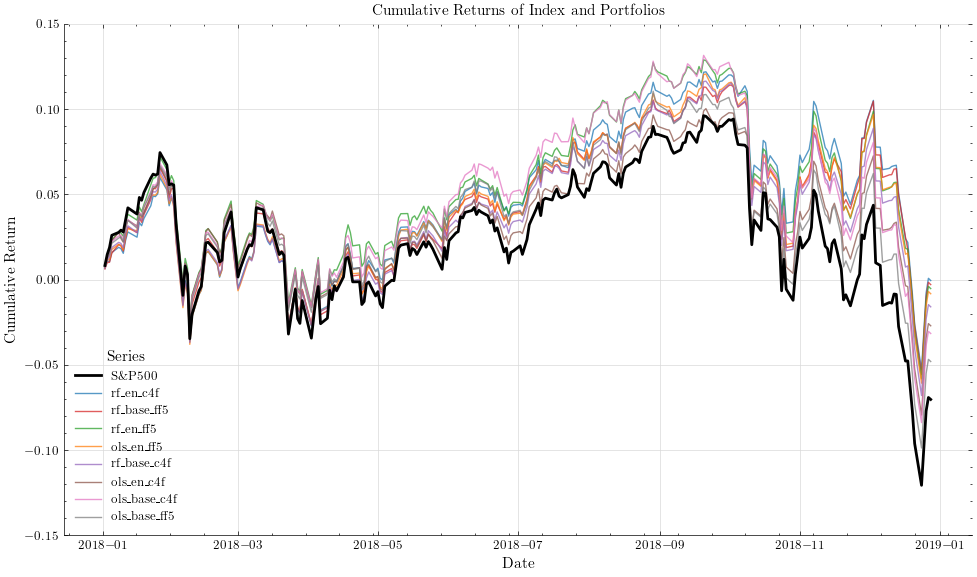
\includegraphics[width=\textwidth]{plots/results/contrained_cum_ret_plot.png}
    \caption{Cumulative returns of S\&P500 and sector rotation strategies (2018)}\label{fig:constr_cum_ret_plot}
\end{figure}

\begin{table}[H]
\centering
\caption{Index and Portfolio Returns: Constrained Strategy}
\label{tab:constr}
\begin{tabular}{lrrrrrrr}
\toprule
{} & \multicolumn{1}{c}{Cumulative} & \multicolumn{1}{c}{Annualised} & \multicolumn{1}{c}{Annualised} & \multicolumn{1}{c}{Alpha} & \multicolumn{1}{c}{Information} & \multicolumn{1}{c}{PSR} & \multicolumn{1}{c}{PSR} \\
{} & \multicolumn{1}{c}{Return} & \multicolumn{1}{c}{Return} & \multicolumn{1}{c}{Volatility} & {} & \multicolumn{1}{c}{Ratio} & \multicolumn{1}{c}{(S*=0)} & \multicolumn{1}{c}{(S*=0.1)} \\
\midrule
S\&P500 & -7.03\% & -7.08\% & 17.06\% & 0.00\% & -- & -- & -- \\
rf\_en\_c4f & -0.05\% & -0.05\% & 15.22\% & 7.03\% & 0.30 & 0.48 & 0.05 \\
rf\_base\_ff5 & -0.29\% & -0.29\% & 15.39\% & 6.79\% & 0.30 & 0.48 & 0.05 \\
rf\_en\_ff5 & -0.52\% & -0.53\% & 15.48\% & 6.55\% & 0.31 & 0.47 & 0.05 \\
ols\_en\_ff5 & -0.83\% & -0.83\% & 15.45\% & 6.25\% & 0.30 & 0.46 & 0.05 \\
rf\_base\_c4f & -1.59\% & -1.61\% & 15.42\% & 5.47\% & 0.29 & 0.44 & 0.04 \\
ols\_en\_c4f & -2.71\% & -2.73\% & 15.43\% & 4.35\% & 0.27 & 0.41 & 0.04 \\
ols\_base\_c4f & -3.16\% & -3.18\% & 15.66\% & 3.90\% & 0.27 & 0.40 & 0.03 \\
ols\_base\_ff5 & -4.80\% & -4.84\% & 15.65\% & 2.24\% & 0.23 & 0.36 & 0.03 \\
\bottomrule
\end{tabular}
\end{table}

\subsection{Discussion}
\subsubsection{Research Questions}

% \begin{enumerate}
%     \item \textbf{Research question 1}\
%     \textit{Does augmenting established linear asset-pricing models with liquidity-risk and sentiment factors, estimated via Random Forests, yield significantly higher out-of-sample explanatory power while retaining interpretability?}
%     \item \textbf{Research question 2}\
%     \textit{Given such an RF-based enhanced factor model, can its forecasts be combined with association-rule learning to derive simple, transparent sector-rotation rules that outperform the S\&P 500 index?}
%     \end{enumerate}

% Research question 1: Does augmenting established linear asset-pricing models with liquidity-risk and sentiment factors, estimated via Random Forests, yield significantly higher out-of-sample explanatory power while retaining interpretability?
% - Including liquidity risk and sentiment factors with Random Forest do yield a significantly higher out-of-sample explanatory power, compare to the baseline linear OLS models. However, it did not yield significantly higher out-of-sample explanatory power, compare to the baseline RF models.
% - Interpretaility approaches , though robust, is not as useful and strong as OLS's approach for financial practitioners. Method suggested by \citeA{simonian_2019}, in this analysis, produces uncamparable results to OLS counter parts, less informative, and lack statistical significance. How ever we could still get there with various alternatives (feature importance, shap, permutation importance) to see effect of each Fama french, liquidity, and sentiment factors on excess returns.
The findings of this thesis partly support the first research question. Enhancing the baseline C4F and  FF5 specifications with liquidity proxies (e.g.\ bid-ask spread, turnover, $ILLQ$) and the time varying sentiment index of \citeA{ung_2024} increases the out-of-sample $R^{2}$ and reduces hold out set forecast errors relative to plain-vanilla OLS benchmarks.  The gains, however, disappear once we benchmark RF against its own variants. It appears the tree ensemble already captures the same non-linearities and that liquidity and sentiment does not seem to significantly add forecasting power to the nonparametric model. In terms of interpretability, global coefficients from OLS remain easier for financial practitioners and managers to digest than feature importances from RF. The pseudo-beta approach proposed by \citeA{simonian_2019} is not only unsuitable for this particular empirical research, it also lacks the statisitcal rigour to be considered a valid substitute. However, when the primary objective is accurate forecasting, model-agnostic interpretability techniques (such as feature importance measures, SHAP values, and partial dependence plots) can elucidate the key drivers of returns in non-parametric models.

Factor attribution reveals a few surprising findings:
- Amihud liquidity, though have been claimed to have effect on excess returns, does not seem to have any effect in our models. \cite{chordia_2017}


% Research Question 2: Given such an RF-based factor model, can its forecasts be combined with association-rule learning to derive simple, transparent sector-rotation rules that outperform the S\&P 500 index?
% - Yes. In both constrained and unconstrained strateies, ARL using RF forecasted rule outperforms S\&P 500 index. Through an empirical test, though we cannot definitely say due to only one year of backtesting, the enhancement factors in random forest models will not harm the performance of the rule-based strategy. Including them is seems to always be better than not. No overfitting/underfitting problems in our dataset. One strong evidence is our enhanced RF models are among the top performing models in the sector rotation strategy. For non-parametric models and for trading purposes, it seems like C4F and FF5 choice entirely depends on macroeconomic factors. 

%todo: Diebold–Mariano maybe?

This paper's approach and its findings support the second research question. Both the unconstrained and turnover-constrained implementations beat the S\&P500 on total return during the 2018 out-of-sample window, with no signs of over- or under-fitting. The inclusion of liquidity and sentiment factors never degrades strategy performance and, in most cases, improves it. The enhanced variant consistently rank among the top performers in the sector rotation strategy. Finally, the relative merits of $C4F$ versus $FF5$ inputs appear to hinge on current macroeconomic conditions rather than on any inherent superiority of one factor set over the other.

In terms of explainability, the framework developed in this paper delivers both the predictive accuracy of non-parametric learners and the transparency afforded by model-agnostic interpretability methods and rule-based trading signals. On any trading day, an individual forecast can be decomposed into the ARL sector rotation rule that generated the signal. That rule itself can be further can be traced back to each allocation decision back to specific Fama-French, liquidity, and sentiment factors via FI rankings (e.g.\ permutation importance or SHAP values), ensuring that every component of the prediction pipeline remains auditable and economically interpretable.

Nevertheless, the evidence should be regarded as preliminary and purely empirical: (i) only a single-year walk-forward evaluation of the expanding-window scheme has been completed, whereas a 20-year rolling back-test is required for robust inference; and (ii) the manual ARL support/confidence thresholds can make the rule set unstable. Replacing ARL with \emph{RuleFit}—a sparse additive rule ensemble—would fuse forecasting and explainability in one algorithm, avoid arbitrary thresholds, and yield naturally interpretable sector signals.

\subsubsection{Limitations}
% - Though we implemented extending window, computing resources limitataitons does not allow me to do 2 decades backtest. Ideally, this analysis should be doen with a proper extending window: train for X numbers of days lookback-> test day after. Then extend window. THen repeat for 20 years. THis paper did do the extending window continous retraining with extending window frame of 1 training year for 20 years. However it is reported as out-of-bag score only. With only 1 year to test out the extending window, it is not ideal. However it got a proxy what the actual result would be.

% - Constraints of ARL: This rule based method is based on manual threshold. Something of recent research, like RuleFit would be better. We are doing RF+ARL -> signals. However Rulefit does not need to be combined with anything else. It could create rules directly as a feature of the algo. These re actual if-then rules, such as "if market return >alpha and turn<= beta and news_sent> gamma then excess_return = 10\%".

% - Cannot statisically proof that either C4F or FF5 is better. But does not seem to entirely matter to non parametric models as we could include both (for forecasting purposes) SHAP, PDP and Feature Importance are only informative, not statisical proofs.
Despite implementing an expanding-window scheme, our back-test remains confined to a single year of walk-forward evaluation due to computational constraints. Ideally, we would train on an initial lookback of $X$ trading days, test on the subsequent day, then extend the training window and repeat this process continuously over a 20-year period. While this paper reports out of bag performance for a one-year training frame across two decades, the absence of a full dataset rolling back test in our study limits the robustness of our conclusions. Our one year proxy, however, suggests that the expanding window approach would likely produce comparable results over a longer time frame.

%TODO RFI: Despite these advantages, two important caveats must be borne in mind. First, local validity is limited: outside the neighbourhood surrounding the point \((x_{1},\dots,x_{p})\), the relationship between factors and returns may differ substantially, so pseudo‐betas should not be extrapolated beyond their local region without caution. Second, the \textbf{independence assumption} underlying the raw elasticities treats factors as if they were orthogonal when computing \(\varepsilon_{k}=\hat y / x_{k}\), which may misattribute explanatory power in the presence of strong interactions. To mitigate this, researchers can group interacting predictors prior to calculating pseudo‐betas or report complementary Shapley‐value attributions to validate and cross‐check the results.  

The ARL relies on manually selected support and confidence thresholds, which may render the extracted “if-then” sector-rotation rules sensitive to arbitrary parameter choices. Recent advances—such as the \texttt{RuleFit} algorithm, which generate sparse, additive rule ensembles directly from the data without the need for external rule mining and threshold tuning. By integrating rule extraction into the learner itself, RuleFit produces concise, interpretable rules (e.g.\ \emph{if} market return $>$ $\alpha$ \emph{and} turnover $\le \beta$ \emph{and} sentiment $>$ $\gamma$, \emph{then} excess return $=10\%$) while avoiding the two-step RF+ARL pipeline.

Finally, we cannot statistically demonstrate that the C4F or FF5 formulations are superior within a non-parametric forecasting framework. In practice, RF models can accommodate both factor sets simultaneously and simply don't split on redudant predictors. Moreover, interpretability tools—feature importance, SHAP values, and PDP—offer descriptive insights into factor contributions but do not constitute formal hypothesis tests. Future work should incorporate inferential procedures (e.g.\ testing differences in out-of-sample $R^2$ or using bootstrap confidence intervals for SHAP contributions) to underpin the economic relevance of each factor choice.

\subsubsection{How investors and asset managers can use the findings of this paper}
% - ideal workflow: gather past data -> plug in -> auto feature engineers_> pipeline (rf -> arl-> rules) -> weighting on tomorrows sector. Tomorrow comes, automatcially include today in traning window, adjust for todays excess returns -> forecast tomorrow -> weight tomorrow..
% - When an actual trade is not as expected -> can go back and see exactly which factor caused the trade to be not as expected with feature importance, shap, pdp
% - With incorporation of sentiment, liquidity risks, can think about other macroeconomic factoers that are less niche, since the two most promonient factors are taken into account. Help financial professional make better decisions that are always explainable at every single step of the trading route
For asset managers, this is the proposed pipeline: automated data ingestion $\rightarrow$ feature engineering $\rightarrow$ RF forecasting $\rightarrow$ rule extraction. This pipeline delivers a daily sector-weight vector whose rationale can be traced factor-by-factor. When live trades deviate from expectations, global and local attribution via feature importance, SHAP, or partial dependence immediately isolates which of the traditional FF factors ($SMB$, $HML$, $MOM$, $RMW$, $CMA$), the liquidity variables, or the sentiment index drove the surprise deviation. Because liquidity risk and sentiment already proxy two of the most pervasive macro drivers, practitioners can next experiment with complementary state variables (e.g.\ term-structure slope, credit spreads) without materially inflating model complexity.


% \noindent\textbf{Recommended refinements and theoretical checks}
% \begin{itemize}
% \item \emph{Statistical testing}: report out-of-sample $\Delta R^{2}$ p-values and Diebold-Mariano statistics to demonstrate that RF-based enhancements are materially better than OLS and not materially worse than vanilla RF.
% \item \emph{Factor choice}: clarify why $C4F$ vs.\ $FF5$ matters once non-parametric learners are used; consider including both sets of factors and letting the algorithm down-weight redundant ones.
% \item \emph{Back-test design}: extend the expanding-window evaluation to the full 1990-2018 span; document walk-forward hyper-parameter tuning to avoid look-ahead bias.
% \item \emph{Interpretability caveat}: remind readers that SHAP and permutation scores are \emph{not} formal statistical betas; they measure marginal predictive contribution, not economic elasticity.
% \item \emph{Liquidity–sentiment theory}: verify that liquidity betas indeed earn a premium during market stress (e.g.\ 2008, 2020) and that sentiment loads interact with the size factor, as implied by \citeA{baker_wurgler_2007}.
% \end{itemize}